\documentclass[12pt]{article}
   
\usepackage[utf8]{inputenc}
   \usepackage{graphicx}
   \usepackage{float}
   \usepackage{subcaption}
   %\usepackage{mathtools}
   \usepackage{amsmath}
   
   \addtolength{\hoffset}{-0.7in}
   \addtolength{\textheight}{1.5in}
   \addtolength{\textwidth}{1.5in}
   \addtolength{\voffset}{-1in}
%
% Title.
\title{EE230: Experiment 3\\
Schmitt Trigger, Monostable, and Astable Circuits}

% Author
\author{Hitesh Kandala, 180070023}

% begin the document.
\begin{document}

% make a title page.
\maketitle

\section{Overview of the experiment}

\subsection{Aim of the experiment}
\begin{itemize}
    \item Design the circuit of Schmitt Trigger and compare the threshold voltages $V_{TH}$  and $V_{TL}$ with the values you expect theoretically. 
    \item Wire up the circuit of astable multivibrator and compare the minimum and maximum period of oscillation with your calculation.
    \item Wire up the circuit of monostable multivibrator and measure the duration of the output pulse. Compare it with your calculation.
\end{itemize}

\subsection{Theory} 
        \begin{figure}[H]
            \centering
            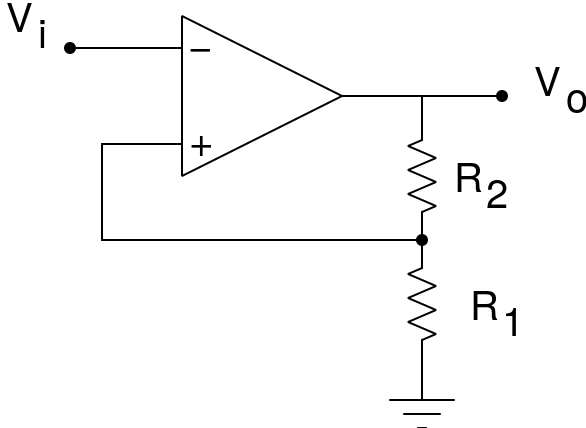
\includegraphics[width = 0.4\linewidth, height = 1.8in]{reports/lab2/non.png}
            \caption{Schmitt trigger}
        \end{figure}
When $V_i$ is sufficiently large, the ouput voltage $V_o$ of the circuit (known as the “Schmitt trigger”) is $−V_{sat}$ as shown in Fig. 1. The voltage at the non-inverting input terminal of the op amp $V_+$ (with respect to ground) is then $V_+ \equiv V_{TL} = −V_{sat}\times(\frac{R_1}{R_1+R_2})$. As $V_i$ is reduced and becomes smaller than $V_{TL}$, the op amp output changes from $-V_{sat}$ to $+V_{sat}$ (since $V_- < V_+$ ). Now, $V_+$ is equal to $V_+ \equiv V_{TH} = +V_{sat}\times(\frac{R_1}{R_1+R_2})$. If $V_i$ is reduced further, this state of affairs continues to hold. If $V_i$ is increased, the output flips when $V_i$ crosses $V_{TH}$.

      \begin{figure}[H]
            \centering
            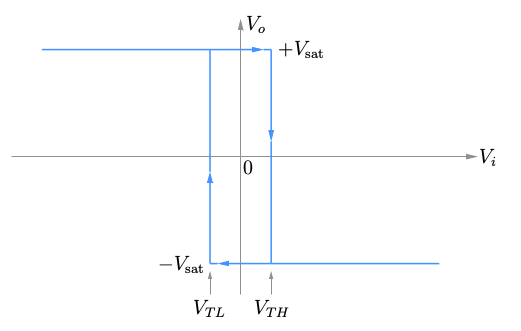
\includegraphics[width = 0.7\linewidth, height = 3in]{reports/lab2/scmiii.png}
            \caption{$V_o$ versus $V_i$ relationship for Schmitt trigger}
        \end{figure}
        \\
        The Schmitt trigger is a comparator with hysterisis (or “memory”). Since the input threshold voltage ($V_{TH}$ or $V_{TL}$), at which the output flips, depends on the “state” of the circuit.
        Note that the high and low threshold voltages, $V_{TH}$ and $V_{TL}$, respectively, are symmetric about 0 V for the Schmitt trigger circuit i.e., $V_{TH} = −V_{TL}$. By connecting a DC voltage source $V_a$ , we can make them asymmetric (see Fig. 3), as shown below.

      \begin{figure}[H]
            \centering
            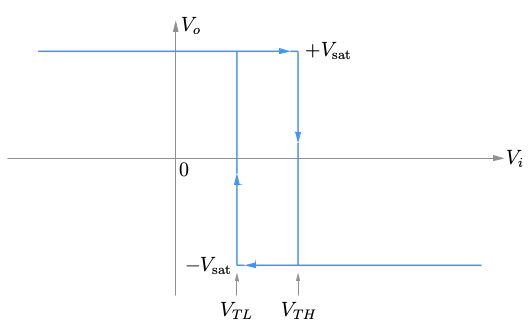
\includegraphics[width = 0.7\linewidth, height = 3in]{reports/lab2/assym.png}
            \caption{$V_o$ versus $V_i$ relationship for the asymmetric Schmitt trigger}
        \end{figure}
        \\
        When $V_o$ is $+V_{sat}$, we have
        \begin{equation}
            V_+ = +V_{sat}\frac{R_1}{R_1+R_2} + V_a\frac{R_2}{R_1+R_2} 
        \end{equation}
        \\
        since the current entering the non-inverting input of the op amp can be neglected. Similarly, when $V_o$ is $−V_{sat}$, we have
        \\
        \begin{equation}
            V_+ = -V_{sat}\frac{R_1}{R_1+R_2} + V_a\frac{R_2}{R_1+R_2} 
        \end{equation}
        \\
        The output voltage of the Schmitt trigger can be limited by using a Zener pair as shown in Fig. 4. Let the breakdown voltage of the Zener diode be $V_Z$ and the turn-on voltage be $V_{on}$. Consider the op amp output $V_{o1}$ to be $+V_{sat}$. Because of the diode pair, the output voltage $V_o$ gets limited to $V_{on} + V_Z$, with $D_1$ in forward conduction, and $D_2$ in reverse breakdown.\\
        \\
        \begin{figure}[H]
            \centering
            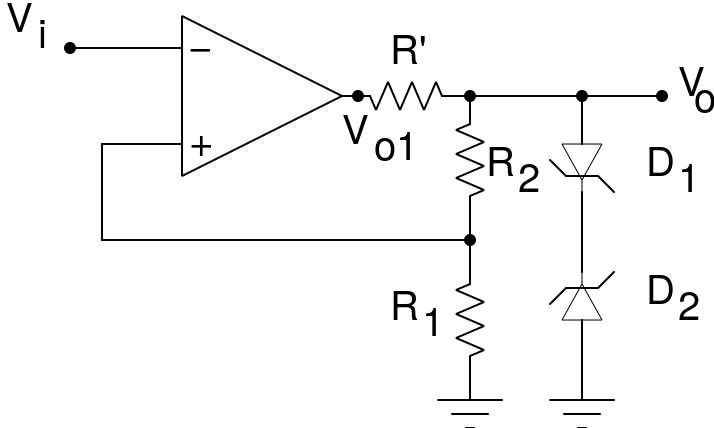
\includegraphics[width = 0.6\linewidth, height = 2.5in]{reports/lab2/zener.png}
            \caption{Schmitt trigger circuit with $V_o$ limited to $±(V_Z + V_{on} )$}
        \end{figure}
        \\
        Note that the difference between $V_{o1}$ and $V_o$ appears across the resistor R which must be chosen to limit the op amp output current to a reasonable value (a few mAs). Connecting the diode pair directly to the op-amp output would lead to unhealthy events. In a similar manner, when $V_{o1}$ is $−V_{sat}$, the output voltage $V_o$ gets limited to $−(V_{on} + V_Z)$, with $D_2$ in forward conduction, and $D_1$ in reverse breakdown.\\
        \\
\newpage
\section{Experimental results}

\subsection{Schmitt trigger}
        \begin{figure}[H]
            \centering
            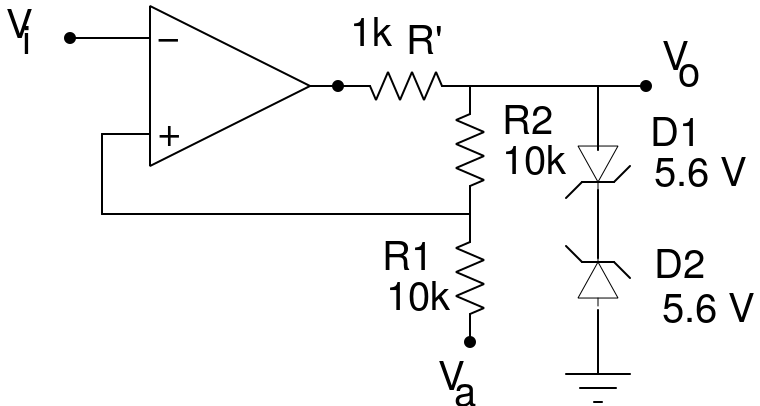
\includegraphics[width = 0.7\linewidth, height = 2.6in]{reports/lab2/scmidt.png}
            \caption{Schmitt trigger}
        \end{figure}
        
        % \begin{figure}[H]
        %     \centering
        %     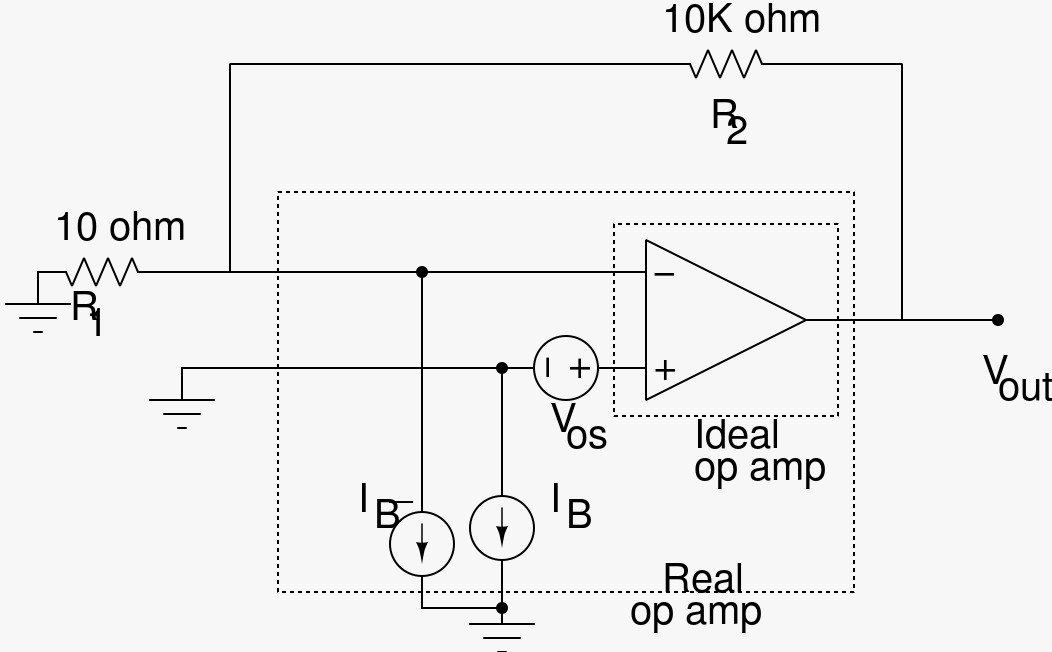
\includegraphics[width = 0.8\linewidth, height = 2.5in]{offset_real.jpeg}
        %     \caption{Equivalent circuit}
        % \end{figure}
      \\
      \textbf{(A) With $\mathbf{V_{a} = 0V :}$}\\
         
        \begin{equation}
            V_{TL} = -V_{sat} \times (\frac{R_1}{R_1 + R_2}) 
        \end{equation}
        \\
        \begin{equation}
            V_{TH} = +V_{sat} \times (\frac{R_1}{R_1 + R_2}) 
        \end{equation}
        \\
        The actual resistance of resistors shown in fig 5 are,
        $R_1 = 9.7k$, $R_2 = 9.82k$, $R' = 0.96k$
        \\
        Drop across zener diodes is $V_{Z} + V_{ON} = 5.6V + 1.12V = 6.72V$\\
        \begin{equation}
            V_{TL} = -6.72 \times (\frac{9.7}{9.7 + 9.82})
        \end{equation}
        \begin{equation}
            \boxed{V_{TL} = -3.34V}
        \end{equation}
        Similarly,
        \begin{equation}
            \boxed{V_{TH} = +3.34V}
        \end{equation}
        \\
        Hence, theoretical values of $\mathbf{V_{TH}}$ and $\mathbf{V_{TL}}$ are \textbf{+3.34V} and \textbf{-3.34V}   respectively.
        \\
        
        \begin{figure}[H]
            \centering
            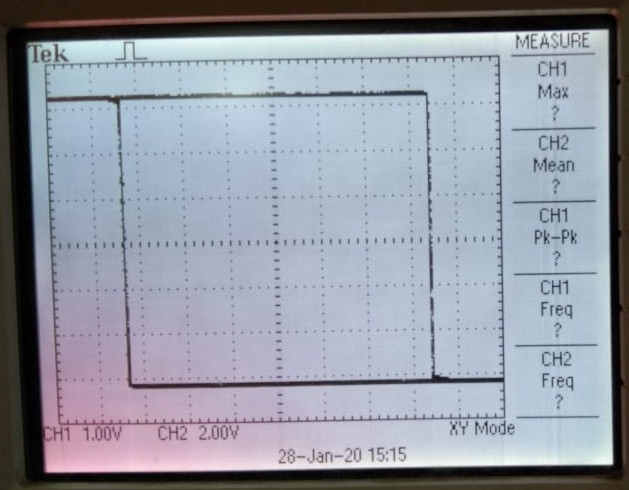
\includegraphics[width = 0.8\linewidth, height = 3in]{reports/lab2/scmidtt.jpeg}
            \caption{$V_o$ versus $V_i$ relationship for $V_a = 0V$}
        \end{figure}
        \\
        The observed value of $\mathbf{V_{TH} = +3.4V}$ and $\mathbf{V_{TL} = -3.4V}$\\
        \\
        \textbf{(B) With $\mathbf{V_{a} = 3V :}$}\\
         
        \begin{equation}
            V_{TL} = -V_{sat} \times (\frac{R_1}{R_1 + R_2}) 
        \end{equation}
        \\
        \begin{equation}
            V_{TH} = +V_{sat} \times (\frac{R_1}{R_1 + R_2}) 
        \end{equation}
        \\
        The actual resistance of resistors shown in fig 5 are,
        $R_1 = 9.7k$, $R_2 = 9.82k$, $R' = 0.96k$
        \\
        Drop across zener diodes is $V_{Z} + V_{ON} = 5.6V + 1.12V = 6.72V$\\
        \begin{equation}
            V_{TL} = -6.72 \times (\frac{9.7}{9.7 + 9.82}) + 3 \times (\frac{9.82}{9.7 + 9.82})
        \end{equation}
        \begin{equation}
            \boxed{V_{TL} = -1.83V}
        \end{equation}
        Similarly,
        \begin{equation}
            V_{TH} = 6.72 \times (\frac{9.7}{9.7 + 9.82}) + 3 \times (\frac{9.82}{9.7 + 9.82})
        \end{equation}
        \begin{equation}
            \boxed{V_{TH} = +4.85V}
        \end{equation}
        \\
        Hence, theoretical values of $\mathbf{V_{TH}}$ and $\mathbf{V_{TL}}$ are \textbf{+4.85V} and \textbf{-1.83V}   respectively.
        \\
        
        \begin{figure}[H]
            \centering
            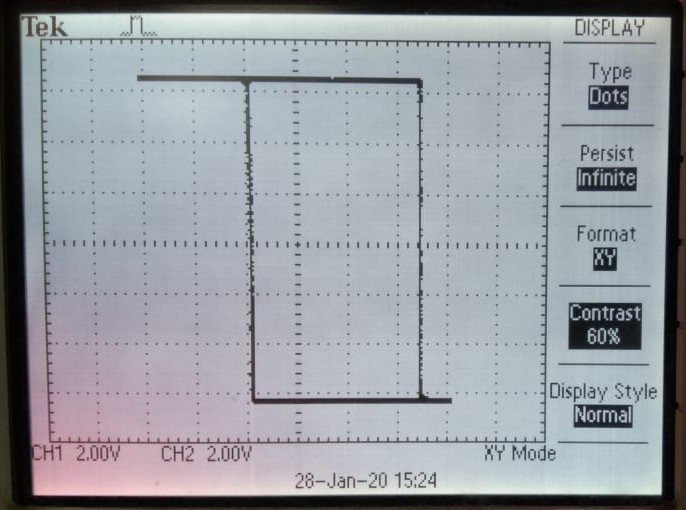
\includegraphics[width = 0.6\linewidth, height = 2.4in]{reports/lab2/scmidtt2.jpeg}
            \caption{$V_o$ versus $V_i$ relationship for $V_a = 0V$}
        \end{figure}
        \\
        The observed value of $\mathbf{V_{TH} = +4.8V}$ and $\mathbf{V_{TL} = -1.8V}$\\

\subsection{Astable multivibrator}
      \begin{figure}[H]
            \centering
            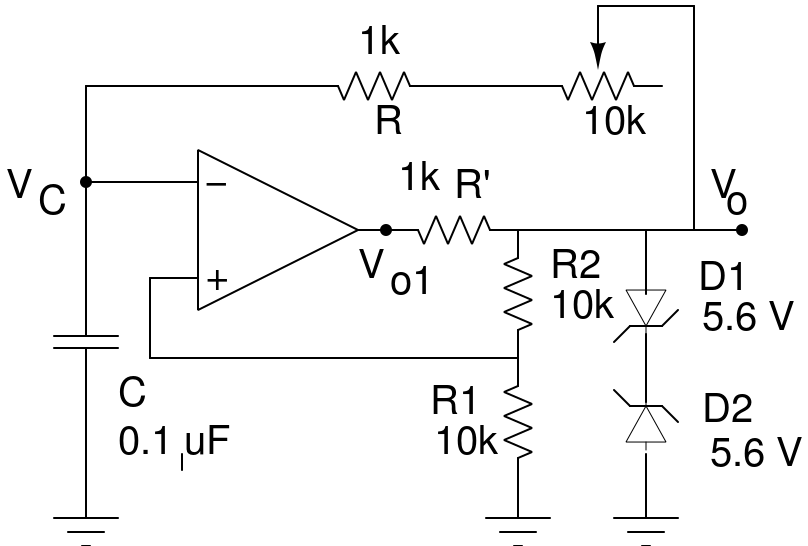
\includegraphics[width = 0.5\linewidth, height = 2.8in]{reports/lab2/astable.png}
            \caption{Astable multivibrator}
        \end{figure}
        \\
        The actual resistance of resistors shown in fig 8 are,
        $R_1 = 9.7k$, $R_2 = 9.82k$, $R' = 0.99k$, $R = 0.96k$\\
        \\
        \textbf{(A) For maximum time period :}\\
        \\
        The resistance between $V_C$ and $V_O$ comes out to be $\mathbf{10.73k \Omega}$
        \\
        Since here $V_a = 0V$,
        % \begin{figure}[H]
        %     \centering
        %     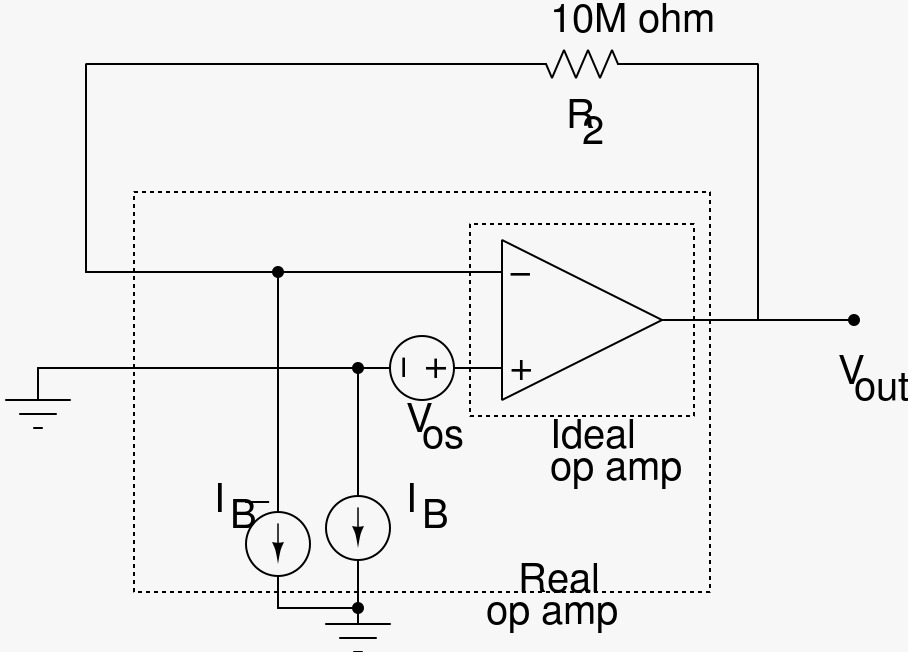
\includegraphics[width = 0.8\linewidth, height = 3in]{ibminusreal.jpeg}
        %     \caption{Equivalent internal circuit}
        % \end{figure}
        \begin{equation}
            V_{TH} = -V_{TL} \equiv V_{T}
        \end{equation}
        \\
        The period of oscillation is
        
        \begin{equation}
            T = 2\tau \log(\frac{V_m + V_T}{V_m - V_T}) \qquad \qquad where \quad \tau = RC
        \end{equation}
        \\
        \begin{equation}
            T = 2(10.73k)(0.1\mu) \log(\frac{6.72 + 3.4}{6.72 - 3.4})
        \end{equation}
        
        \begin{equation}
            \boxed{T = 2.39ms}
        \end{equation}
        \\
        \begin{figure}[H]
            \centering
            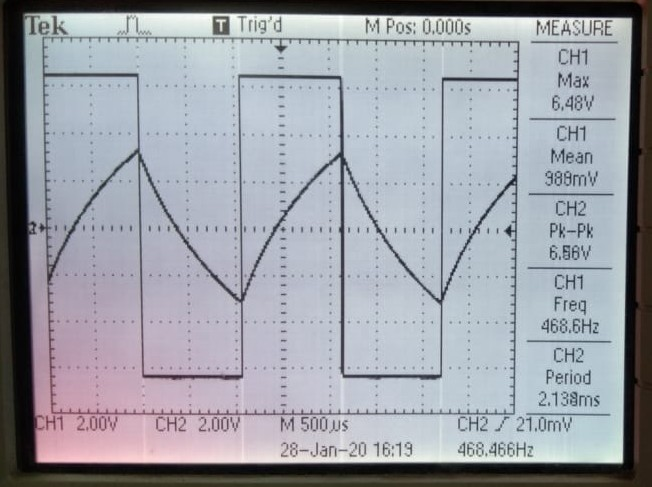
\includegraphics[width = 0.6\linewidth, height = 2.5in]{reports/lab2/astable.jpeg}
            \caption{Output for maximum time period}
        \end{figure}
        \\
        The observed maximum time period is $\mathbf{T = 2.138ms}$\\
        \\
        \textbf{(B) For minimum time period :}\\
        \\
        The resistance between $V_C$ and $V_O$ comes out to be $\mathbf{0.96k \Omega}$
        \\
        Again, the period of oscillation is given by
        
        \begin{equation}
            T = 2\tau\times \log(\frac{V_m + V_T}{V_m - V_T}) \qquad \qquad where \quad \tau = RC
        \end{equation}
        
        \begin{equation}
            T = 2\times(0.96k)\times(0.1\mu)\times \log(\frac{6.72 + 3.4}{6.72 - 3.4})
        \end{equation}
        
        \begin{equation}
            \boxed{T = 214\mu s}
        \end{equation}
        \\
        \begin{figure}[H]
            \centering
            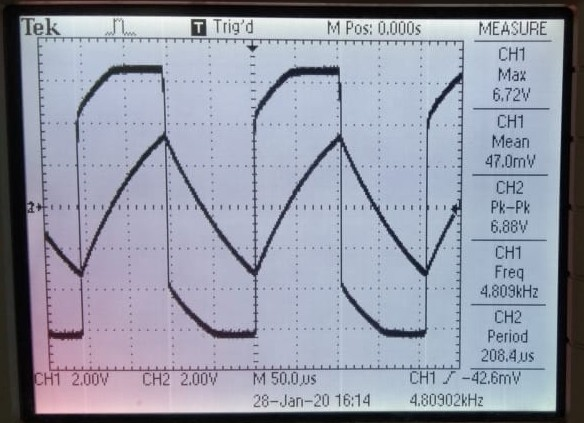
\includegraphics[width = 0.6\linewidth, height = 2.5in]{reports/lab2/astableMin.jpeg}
            \caption{Output for minimum time period}
        \end{figure}
        \\
        The observed minimum time period is $\mathbf{T = 208.4\mu s}$\\

      \subsection{Monostable multivibrator}
      \begin{figure}[H]
            \centering
            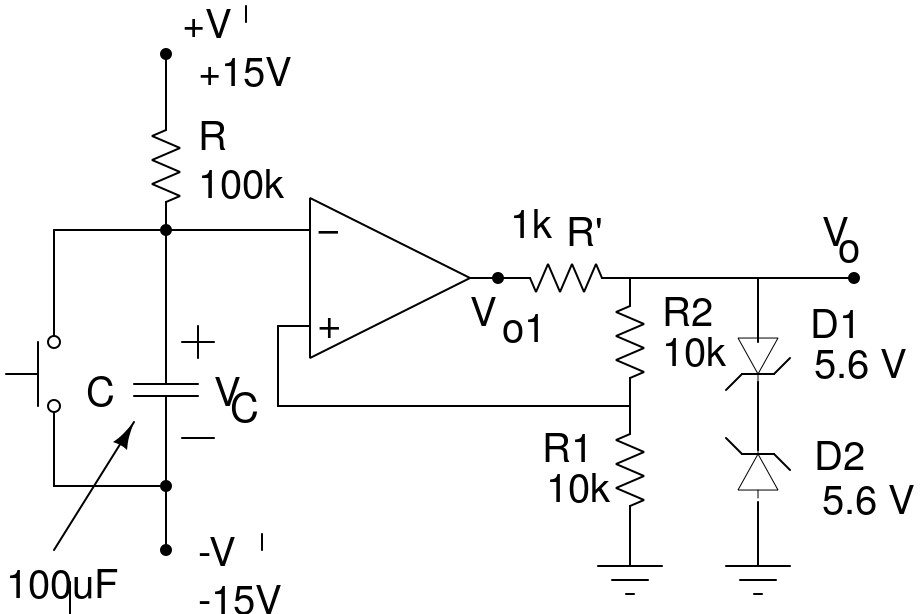
\includegraphics[width = 0.6\linewidth, height = 3in]{reports/lab2/mono.png}
            \caption{Monostable multivibrator}
        \end{figure}
       The actual resistance of resistors shown in fig 11 are,
        $R_1 = 9.7k$, $R_2 = 9.82k$, $R' = 0.99k$, $R = 100.5k$\\
        The voltage to which the capacitor charges is $2V' = 10.6V$\\
        \newpage
    The output pulse width, T is given by the expression
      \begin{align*} 
            T & = RC \times \log(\frac{V'}{V'-V_{TH}})\\
              & = (100.5k)\times(100\mu)\times\log(\frac{5.3}{5.3-3.4})
      \end{align*}
      \begin{equation}
            \boxed{T = 10.25s}
      \end{equation}
      
      \begin{figure}[H]
            \centering
            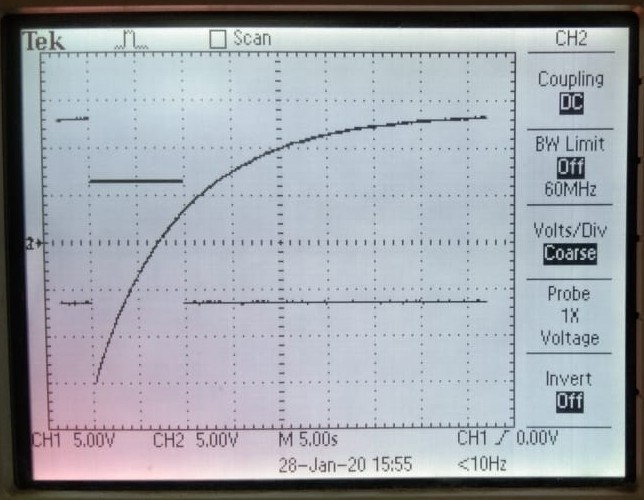
\includegraphics[width = 0.6\linewidth, height = 3in]{reports/lab2/monostable.jpeg}  
            \caption{Waveforms of $V_{-}$ and $V_{o}$}
        \end{figure}
      \\
    The observed pulse width comes out to be $\mathbf{T = 10.1s}$ 

\vspace{4cm}

    \begin{thebibliography}{9}

        \bibitem{Analog LAB Manual} 
        Scmitt supporting document 
        \\\texttt{https://moodle.iitb.ac.in/pluginfile.php/302403/mod\_resource/content/0/\\schmitt\_astable\_support.pdf}
        % \bibitem{Datasheet of UA741}
        % Datasheet of OpAmp UA741
        % \\\texttt{https://www.slideshare.net/YongHeuiCho/u-a741}
        
    \end{thebibliography}

\end{document}

